% !TEX root = ../2021_microservices_wileytemplate.tex

\section{Results}\label{sec:results}

In this section, we present the results from our systematic literature review. First, we show a general overview of the collected paper's characteristics (Section~\ref{sec:results-general}). Then, we present our results to answer our first research question related to challenges (Section~\ref{sec:results-rq1}). Finally, we describe our findings to answer our second question on the topic of technologies (Section~\ref{sec:results-rq2}).

\subsection{General Analysis}\label{sec:results-general}

Figure~\ref{fig:collected-papers-slr} shows an overview of the collected literature references we used in our systematic literature review. In our study, we have a total of 81 references, of which 60 are from scientific sources and 21 come from grey literature. 

\begin{figure*}[h]
    \centering
    \begin{subfigure}[b]{0.40\textwidth}
        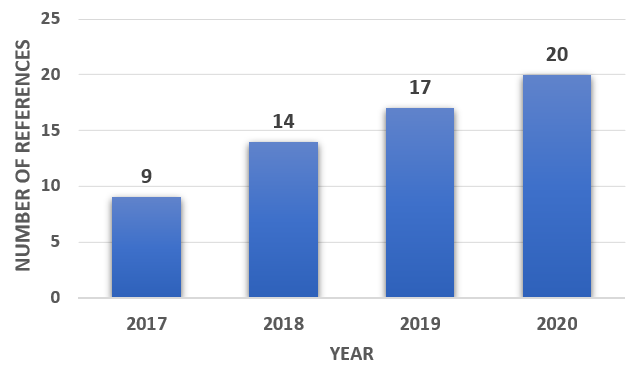
\includegraphics[width=\textwidth]{images/publicationtypes_1.png}
        \caption{Scientific references per year}
        \label{fig:papers-academic-year}
    \end{subfigure}
~
    \begin{subfigure}[b]{0.25\textwidth}
        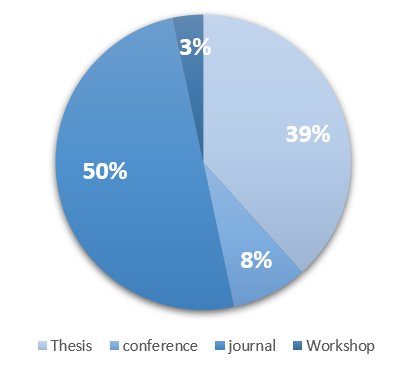
\includegraphics[height=0.2\textheight]{images/publicationtypes_3.png}
        \caption{Types of the scientific references}
        \label{fig:papers-academic-type}
    \end{subfigure}

    \begin{subfigure}[b]{0.40\textwidth}
        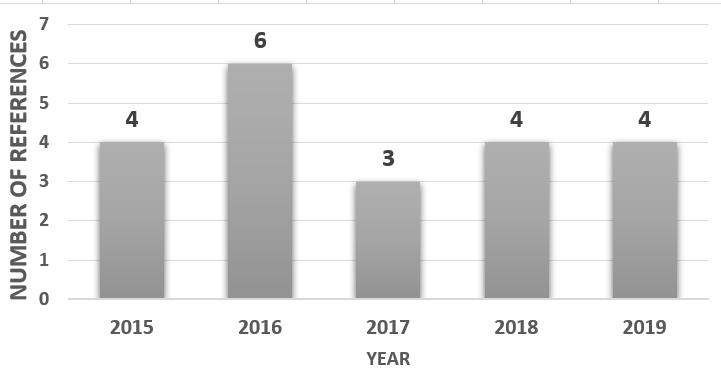
\includegraphics[width=\textwidth]{images/greytype_1.png}
        \caption{Grey references per year}
        \label{fig:papers-grey-year}
    \end{subfigure}
~
    \begin{subfigure}[b]{0.25\textwidth}
        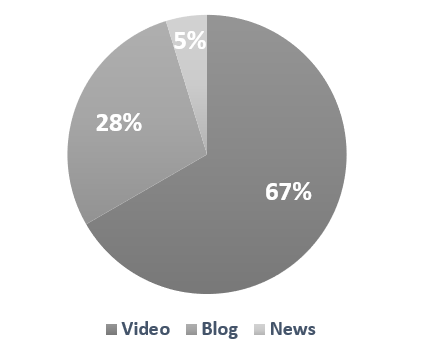
\includegraphics[height=0.2\textheight]{images/greytype_2.png}
        \caption{Types of the grey references}
        \label{fig:papers-grey-type}
    \end{subfigure}

    \caption{collected references Used in the systematic literature Review}\label{fig:collected-papers-slr}

\end{figure*}


We can see the number of scientific references we deemed relevant for our study to grow each year after 2017 (Figure~\ref{fig:papers-academic-year}). Even though we reject papers from before 2017 from our study, we did not design our remaining selection criteria to favor more current papers. Therefore, the rise in the number of references per year is probably just a coincidence. 
%In Figure~\ref{fig:selected-papers-slr-1} We can see the number of papers published after 2017 and the number is growing more every year. In Figure~\ref{fig:selected-papers-slr-2} We can see here the types of publications collected during the SLR \henrique{These are questionable remarks. Since you selected these papers, you cannot claim a generalized trend or a raise.}\keerthana{fixed it}
%
On the other hand, most of the grey literature we used in this study is from 2016 (Figure~\ref{fig:papers-grey-year}). The reason is that the goto conference was our initial starting point to collected grey references. Particularly in 2016, many speakers were discussing microservices in the goto conference.

When we look at the types of literature, we have different classifications for scientific (Figure~\ref{fig:papers-academic-type}) and grey (Figure~\ref{fig:papers-grey-type}). Since all scientific references were papers, we classified them by their publication type (e.g., journal paper, conference paper, thesis). For grey, we classified the references by their media type and publishing format (e.g., video, blog). 
%
%Figure~\ref{fig:selected-papers-grey-1} shows the types of grey literature collected year-wise. There was a total of 21 grey literature which includes blogs, Youtube videos, and News. We could see that there was a lot of grey literature initially published and this serves as a key for practitioners or academia to learn from it and start making more grey literature.
%
From the selected references, we could see there is a good variety of publications. %This may indicate that microservices are discussed in many fields for both the industrial and academia.


\subsection{RQ\#1: What are the main challenges when adopting microservices?}\label{sec:results-rq1}

\begin{figure*}[t]
	\centering
	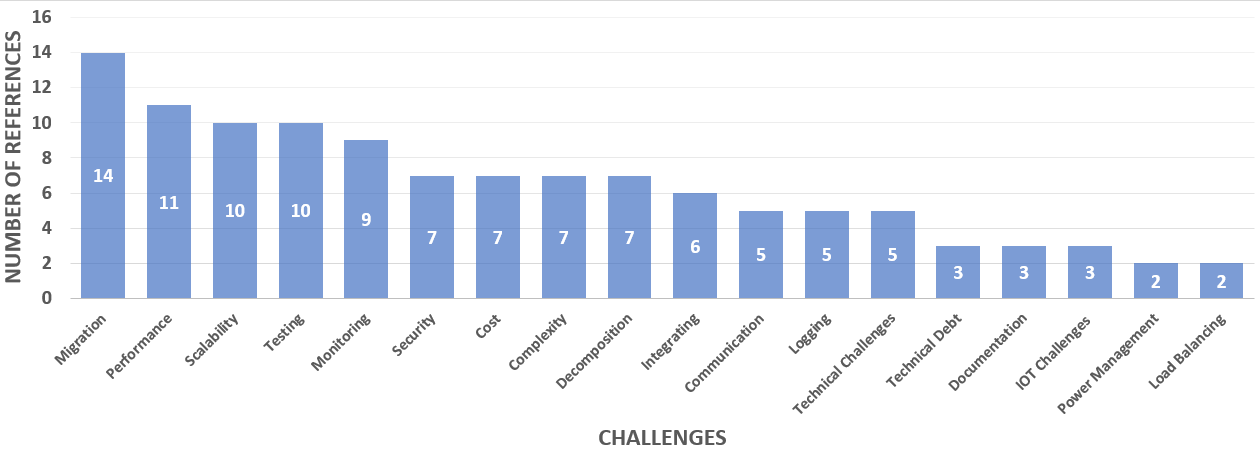
\includegraphics[width=0.9\linewidth]{images/Challenges_updated.png}
	\caption{Challenges in adopting microservices }
	\label{fig:challenges}
\end{figure*}	

In this section, we answer our first research question by analyzing the collected data.
To answer RQ\#1, we examined the spreadsheets created in the data synthesis phase from our 81 references.

Figure~\ref{fig:challenges} shows the challenges in adopting microservices that we discovered in our systematic literature review. It also shows how many distinct references in our selection discuss such challenges. 
According to our classification, we identified \challengecount challenges.
The challenges mentioned on the most number of references are migration and performance, followed by scalability and testing. In our collected data, those are the major challenges of adopting microservices. Next, we focus in more detail the top-10 challenges.


\subsubsection{Migration}%#1
When migrating an application updating the codebase is a difficult task.\cite{Tuuli2020, wang2020}
Another main concern is the risks associated with an application with a database, and how to perform the database migration, especially its location inside a container (e.g., Docker).
Moreover, hosting service migration is seen as also a problem due to the uneven server load, as well as the difficulty of applying updates to the application.\cite{Tuuli2020}

Many organizations are planning and migrating their on-premise software to the cloud, starting with the Infrastructure as a Service (IaaS) and Software as a Service (SaaS) models. Nonetheless, they are facing some challenges and difficulties, mainly in the Platform as a Service (PaaS) model, related to the complexity in integrating the legacy and internal systems.\cite{rosa2018} It requires a different way of thinking compared to the traditional way of software architectures, often leading to the migrations and creations of these architectures being long and costly processes.\cite{Leo2019}

% System application migration is becoming an emerging issue with different challenges. Migration of the system to microservice optimizes decentralization, replaceability, and autonomy of software architectures. Although researchers are not convinced of any specific definition of microservice, its modeling techniques, and its properties, it is aware of system migration to microservices~\cite{ghayyur2018}.

Migration of the resulting application towards the new intended state is still a (partially) manual and labor-intensive step.\cite{overeem2018} If on the one hand microservices can help in achieving a good level of flexibility (e.g., by promoting low services coupling, higher maintainability), on the other hand adopting a microservice-based architecture may bring higher complexity.\cite{Difrancesco2017} %The microservice architectural style has become an essential element for the development of applications deployed on the cloud and for those adopting the devops practices. Nevertheless, while microservices can be used to develop new applications, there are monolithic ones, that are not well adapted neither to the cloud nor to devops. Migrating these applications towards microservices appears as a solution to adapt them to both. 

%Companies have been widely investing in modernizing the software architecture and development processes of their products. By migrating away from software monoliths towards the emerging microservice architecture style, an agile and robust software system with a compatible development process can be accomplished. Despite this, modernization can be highly challenging from a practical point of view. Available software solutions, which aim at supporting the restructuring of software monoliths into microservices, often do not satisfy the arising demands of the developers. While these products offer diverse static analysis functionalities, dynamic analysis aspects are mostly missing. Yet, especially a dynamic analysis can provide invaluable information about overlooked characteristics of the software system~\cite{Lenga2019}.

Serious efforts have been taken to move from monolithic architectures to microservice architectures. A common problem in these efforts is to identify which components from monolithic applications are the best candidates to turn into microservices. It is a tiresome manual effort that requires analyzing many dimensions of software architecture views and often relies on the experience and expertise of the expert performing the extraction.\cite{Kamimura2018, selmadji2020}

\subsubsection{Performance}%#2

Goldsmith~\cite{Kevin2015} talks about challenges related to monitoring, latency, and problems with completely autonomous teams. The distributed aspect of a microservice system is a significant challenges.\cite{Matt2016} Its distributed nature impacts the performance of the system. Calls to a single service might trigger a cascade of additional calls to other services distributed across a network, each adding its latency. The increase in resource usage may cause a microservices-based application to execute slower.\cite{Etsy, Netflix} It can be hard to achieve the same level of performance as with a monolithic approach because of latencies between services. The communication between multiple microservices can introduce performance issues if the services are too fine-grained.  

REST APIs are favored by microservices developers, but there is a concern over its effect on performance when the client-side application grows.\cite{Ghebremicael2017} Experiments reported that the performance of a microservice model is lower than a monolithic model.\cite{Johansson2019} The complex dependencies between services bring new challenges to the monitoring analysis and quality assurance of system performance.\cite{Zhihui2020} Moreover, monitoring the performance of the microservices is still challenging.\cite{Saman2017, Venugopal2017}

%Although microservice offers opportunities for accommodating ever-growing workloads in the cloud, its true scalability potential has not been exploited yet. The reason behind this is the heterogeneity of microservices is never well exposed to the data center management layer, unavoidably causing power allocation imbalance and power capacity waste. Oftentimes, they overlook the sensitivity of performance to power budgeting of each microservice. As a result, it could waste precious power budget on some less critical microservices while leaving inadequate power budget to the most important ones~\cite{Hou2019}. Ensuring our application runs smoothly post-migration, and that the user experience was not negatively impacted, we need a way to compare performance metrics from pre-and post-migration and this can be very difficult.


\subsubsection{Scalability}%#3

The versatility of microservices is one of its finest characteristics, but it comes at a price. Scaling can involve handling several different components and services. This means that either all the components need to scale at the same time, or we need means of identifying which individual components to scale up, and a method of ensuring it.\cite{Meshenberg2016}
%
The hindrance of how to most effectively and efficiently auto-scale a web application to optimize for performance while reducing costs and energy usage is still a hurdle. In particular, this problem has new relevance due to the continued rise of internet of things and microservice-based architectures. A key concern, that is often not addressed by current auto-scaling systems is the decision on which microservice to scale to increase performance.\cite{coulson2020}

Microservices require a different approach to monolithic systems when it comes to scaling. For microservices, one needs to consider both the individual components and the system as a whole. Doing so requires that the dependencies of each microsystem also scale with it.
A modern and successful microservice system can expect a steady rise in traffic, and therefore resource demands, overtime.\cite{Etsy, Soundcloud}
%Scaling a website to handle more traffic at peak times without wasting resources~\cite{McElhiney2018} is extensive research to any web company that has issues with rising costs as demand for their website increases. 
Some of the scalability challenges include enabling efficient scaling and high availability for services for the business requirement. Each module having different scalability criteria could be overpowering.\cite{khan2020}



\subsubsection{Testing}%#4

In contrast with a monolithic architecture, it is easier for microservices to test small, independent components. However, testing microservices can become challenging, particularly the integration tests.\cite{Dmitrii2019} Some industrial blogs claimed that testing can be the biggest challenge with microservices.\cite{Soundcloud, Karma}

To write an effective integration test, the quality assurance engineer should have good knowledge of each of the services that are a part of the test case. Another reason why testing a microservices-based application is difficult is because such applications are generally asynchronous. It is challenging to estimate the reliability of microservices, which is difficult to perform before release due to frequent releases/service upgrades, dynamic service interactions.\cite{Russo2020} 

Nevertheless, testing the system, in general, becomes more challenging. A large number of integrational tests should be implemented to verify that the system is correctly working.\cite{Zaytev2018} Splitting a single process application into multiple services causes the testing process to be more challenging.\cite{Huttunen2017}
"It has been an incredible challenge getting failure testing instilled as a requirement" claimed Ranney.\cite{Matt2016}
%
Korbes\cite{Ellen2018} stated "I want my monolith back!" to demonstrate the sentiment often echoed because developing multi-service, multi-container systems in Kubernetes environment which lacks a lot of the convenience monoliths used to have.
%Straight-forward builds, trivial testing between components is needed. 



\subsubsection{Monitoring}%#5


Monitoring one application running in multiple instances is easier than monitoring multiple services running in multiple instances. Typically with microservices, the number of instances is much higher than with monoliths.\cite{Kalske2017paper} Compared with the traditional monolithic architecture, the microservice architecture style divides a system into different microservices that run in the distributed system. The complex dependencies between services bring new challenges to the monitoring analysis and quality assurance of system performance.\cite{Zhihui2020, Venugopal2017}

%The traditional forms of monitoring and diagnostics will not align well with microservices since we have multiple services working together to make up the same functionality previously supported by a single application.
When a problem arises in the application, finding the root cause can be challenging. If we do not have a means of monitoring and tracking the path a specific request took, like how many and which microservices were traversed for a specific request coming from a user interface. Monitoring systems now need to provide integrations with a large and dynamic ecosystem of third-party platforms to provide complete observability.\cite{Netflix} In containerized workloads, we have to monitor multiple layers, dimensions, and the power consumption it makes.\cite{Kristiani2020} Microservices require continuous and automated monitoring.

Microservice monitoring brings specific challenges. They are often short-lived, which means monitoring over a longer period can be more complicated, and there may be more pathways through which the service is reached, potentially exposing issues such as thread contention.\cite{Zhang2019} Monitoring microservices can be a key factor to detect service failure earlier. However, few studies have been done on monitoring and analysis of microservice performance.\cite{Saman2017, Monterio2018}
%Although powerful tools exist for monitoring microservices, they are usually complex and suitable for monitoring large and complex microservice systems.
%The dashboard is also too complex so it makes the tools not easy to understand for novice users~\cite{Utomo2020}.

\subsubsection{Security}%#6

The implementation of microservices might introduce new security challenges. Each separate service must be able to communicate and interact with the other and this is achieved through the cloud. It is simple to see how this architectural model can impact security. We have moved from securing a single application kept within a single operating system to a multiplicity of parts dispersed in a distributed environment. There is a greater area for attack.\cite{Zaytev2018} Microservices is triggering a closer interaction between the development and operation teams to support the applications lifecycle. Both development and operations need to have a good understanding of the processes involved and to ensure any security risks can be reduced.\cite{Aaron2018,Amazon,Gonchar2017}

%Data generated in a microservices architecture moves, changes, and is continuously interacted with. Data is also stored in different places and for different purposes. Owners of data assets need insight into the life cycle and the dynamics of data to avoid breaches. Data leaks might happen~\cite{tenev2019}. Security is a major challenge that must be carefully thought of in microservices architecture. Services communicate with each other in various ways creating a trust relationship.
Data security is also a concern with microservices applications, as each service can have a different data source. Owners of data assets need insight into the life cycle and the dynamics of data to avoid breaches. Data leaks might happen.\cite{tenev2019}

%For some systems, a user must be identified in all the chains of service communication~\cite{Monterio2018}.

\subsubsection{Cost}%#7
'Scalability comes with costs' states Koschel et al.\cite{Koschel2017}  because communication between microservices becomes more complex. It is no longer possible for components to communicate with each other via simple method calls. %Instead, inter-process communication mechanisms are required. 
This has an impact on how to design the interfaces. 
%Method calls are fast and can be made often without running into any problems. But 
Remote calls are expensive and have high latency compared to simple method calls.\cite{Koschel2017, McElhiney2018}

%From the survey by Zhang et al, we understand that microservices can handle multiple diversity of technology stacks however, the cost of setting up the technical framework was expensive and it took developers a long time to cope up with the obstacles of excessive technology stacks. Foreign technologies and tools spent much effort and cost on setting one by one. To understand the legacy system the practitioners have no choice but to rely on the costly manual code reading and analysis of the dependency among components ~\cite{Zhang2019}.

The complexity of supporting both the microservice and the monolith will linger for a long since it takes a long time to entirely replace the monolith. The longer the migration process takes, the more it costs to maintain the two infrastructures.\cite{Meshenberg2016, Michael2018, Ndungu2019}

In the survey by Leo et al.,\cite{Leo2019} the participants mentioned that respondents seem reluctant on migrating towards a microservice architecture because of the reasons that microservices are complex, new, not yet standardized enough, and that the migration is too costly and time-consuming.

%Depending on where we are starting from, the getting started costs might be a budget concern. we need a large group of developers to set up a complex ecosystem, meaning the cost of getting started can be higher with microservices than with a monolith. Because it is split into very granular microservices, even minor change requests can require us to change several services~\cite{McElhiney2018, Ndungu2019} leading to a duplicated cost of changes. Chaotic independence, unguided organizational transformation, complexity of API management, excessive technology diversity, data inconsistency, unsatisfying monitoring and logging, and inadequate automation are an addition to the costs~\cite{Zhang2019}. Non-technical challenges arise during shift, microservices comes with cost~\cite{Koschel2017,Meshenberg2016,Michael2018}


\subsubsection{Complexity}%#8

%Microservices might sound simple as separate individual services but it is the place for complexity.
Designing microservices that tackle the complexity not only of the services but of the system as a whole is challenging because a microservice-based application is a network of different services that often interact in ways that are not obvious. The overall complexity of the system tends to grow. Many organizations are moving from on-premise software to the cloud but they are facing some challenges and difficulties mainly in the Platform as a Service (PaaS) model, related to complexity in integrating legacy and internal systems.\cite{rosa2018, Zaytev2018}

The adoption of microservices does not reset a system's development and maintenance complexity but is often viewed as a tradeoff between inner and outer complexity. Microservices make complexity more visible and unambiguous hence facilitating its proper handling and management. This represents a total shift in complexity from inside the services to the connections between them and their management.\cite{Ndungu2019, gozneli2020}

Microservices add complexity to the application architecture because of the sheer number of moving parts, hence without automation and the use of DevOps model which encourages continuous integration, continuous delivery, and provisioning, etc., it is very challenging to manage microservice-based applications. Without adopting DevOps culture, organizations will not be able to realize the value of microservices.\cite{Premchand2018}

%With a growing focus on adopting microservices, developers often find it frustrating when someone modifies an application programming interface in a microservice. It is incredibly difficult to fully understand the impact of that change, which makes it difficult to throw blame around. It is a complex task to search through all microservices calling that application programming interface~\cite{Branko2018}.


\subsubsection{Decomposition}%#9

Decomposing a system into independent subsystems is a normal process in software engineering.
The decomposition of systems took on another dimension, especially due to microservices.\cite{Netflix, Fred2015} In microservices, every module is developed as an independent and self-contained service. Decomposing a monolithic system into microservices is a critical and complex task and several practitioners claim the need for a tool to support them during the slicing phase to identify different possible slicing solutions.\cite{Taibi2019} Most often, the decomposition is performed manually by software architects.\cite{Zhang2019, Carvalho2019}
One of the main challenges is to design microservice and creating services that are not too large or too small and contain the right amount of functionality. Many authors proposed domain driven design (DDD) as the best modeling approach that could help overcome this challenge of designing. However, how to apply this idea in practice is not clear to everyone.\cite{Merson2020}

%It can be determined that the fine-grained splitting of the microservice framework can promote the reasonable sharing and effective integration of data. However, how to determine the granularity of microservice splitting is a multiparameter and multiobjective decision-making problem, which is also a key basic problem to be solved urgently both in academic research and application~\cite{Yan2020}.


\subsubsection{Integrating}%#10

The microservices architecture fosters building a software application as a suite of independent services.\cite{rosa2018} When we have to realize a given business use case, we often need to implement the communication and coordination between multiple microservices. Therefore, integrating microservices and building inter-service communication have become challenging tasks.

%It is not recommended to tie the integration between services to some specific technology, because developers might want to use different programming languages when implementing services.
There are also multiple additional challenges when thinking about the integration of microservices. The interface of microservice should be simple to use and it should have good backward compatibility so when new functionalities are introduced, the clients using the service do not have to be necessarily updated.\cite{Kalske2017paper, Zhang2019, liu2018} The integration of the model environment and the runtime environment is essential to achieving fine-grained evolution.\cite{overeem2018}




\subsection{RQ\#2: What are the main technologies or solutions used for implementing microservices?}\label{sec:results-rq2}

\begin{figure}[h]
	\centering
	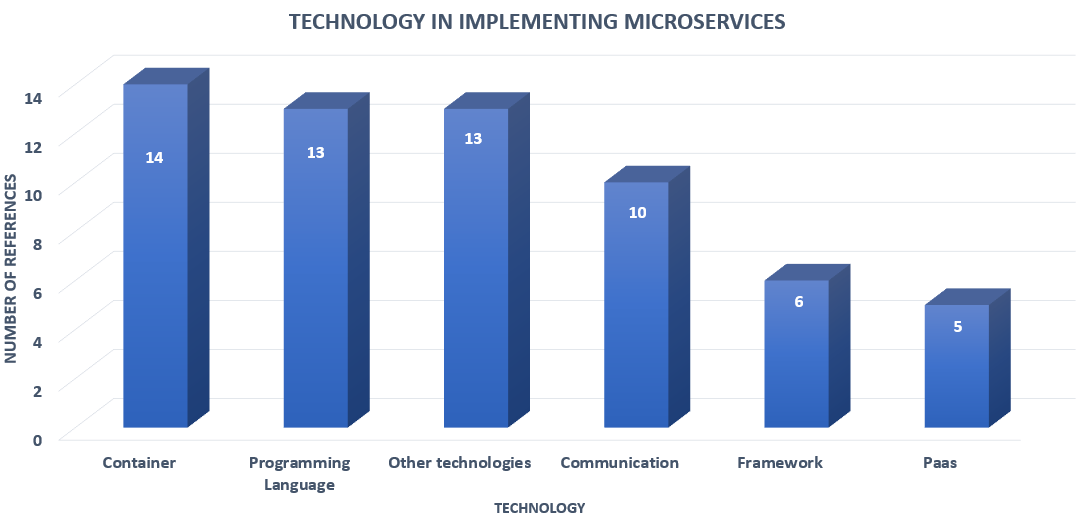
\includegraphics[width=0.65\linewidth]{images/commtechother.png}
	\caption{Technologies per group used for Implementing Microservices}
	\label{fig:tech-group}
\end{figure}	

In this section, we discuss RQ\#2, which is about the technologies used in the implementation of microservices according to our studied sources. Figure~\ref{fig:tech-group} shows the major groups of technologies that appeared in our studied references. We classified the technologies into \techgroupcount major groups.
Figure~\ref{fig:tech-distinct} shows the distinct technologies proposed to implement microservices. In total, we discovered \techcount different technologies in our data. 
The number of references of the groups showed in Figure~\ref{fig:tech-group} is the union of the references of the distinct technologies (Figure~\ref{fig:tech-distinct}) we classified in each group.  

\begin{figure*}[t]
	\centering
	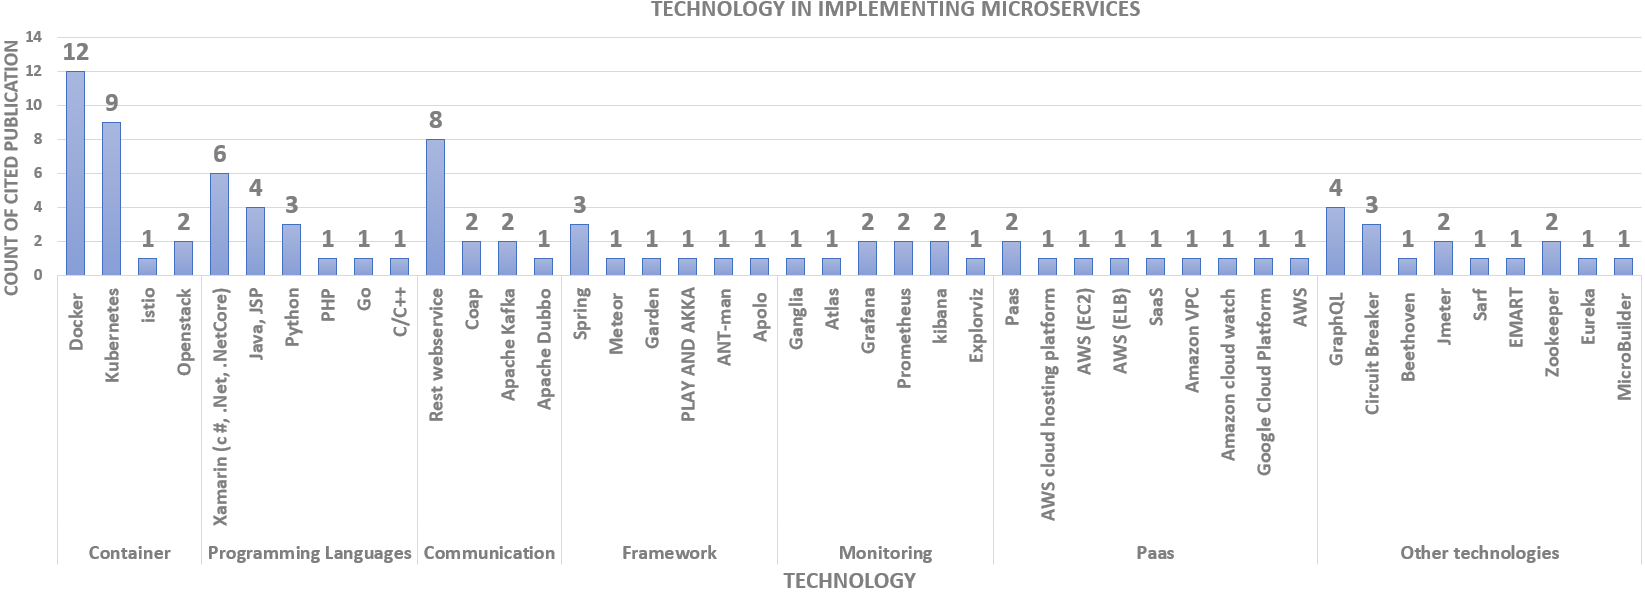
\includegraphics[width=\linewidth]{images/commontechupdated.png}
	\caption{Technologies in implementing microservices }
	\label{fig:tech-distinct}
\end{figure*}


\subsubsection{Containers}
Containers encapsulate discrete components of applications provisioned only with the minimal resources needed to do their job. Containers and microservices enable developers to build and manage self-healing service-based applications more easily.

Docker is a platform for implementing and deploying applications. Developers can implement applications very fast by using docker.\cite{khan2020, Kristiani2020, Sharaf2019} Moreover, it is simpler to create required services separately and manage them as microservices without affecting other services.\cite{Leo2019, Kalske2017paper, Hou2020, Bahadori2018} We can create a docker image for service and view our microservice application inside a docker container. Docker swarm applications can be deployed as services in a swarm cluster.\cite{Venugopal2017, coulson2020, Falatiuk2019}
	
Kubernetes is a container orchestration system that is well-suited to automate the management, scaling, and deploying of microservice applications.\cite{khan2020, Zaytev2018, Kristiani2020}
%It is also possible to run kubernetes locally using MiniKube.\cite{Leo2019, Kalske2017paper}
Kubernetes ensures that the desired state (i.e., the state that we want the system to be in) and the actual state (i.e., the state that the system is actually in) are always in sync. Kubernetes continuously monitors the health of the cluster and ensures that the system is self-healing.\cite{Venugopal2017, Bahadori2018, Falatiuk2019}

Red hat openshift is an open-source container application platform based on the kubernetes container orchestrator for enterprise application development and deployment.\cite{Johansson2019, Bahadori2018}


\subsubsection{Programming Language}
When it comes to microservices development, a natural question is what language to choose. Developers have many options regarding programming languages to develop microservices. Microsoft's Xamarin (C\#, .Net) with Asp.net offers built-in support for deploying microservices using Docker containers.\cite{Johansson2019, liu2018, Falatiuk2019, chauvel2018, haugeland2020, neves2019} Other languages solutions for implementing microservices includes Java WSO2MicroservicesFramework,\cite{Venugopal2017, khan2020, Sharaf2019, KalskeM2017} and Python's flask application.\cite{Ghebremicael2017, khan2020, Hou2020}

%Xamarin (C\#, .net, .netcore) makes it easy to create the application programming interface to become microservices. Asp.net comes with built-in support for developing and deploying your microservices using docker containers.\cite{Johansson2019, liu2018, Falatiuk2019, chauvel2018, haugeland2020, neves2019}

%For Java, WSO2MicroservicesFramework is a solution for implementing microservices.\cite{Venugopal2017, khan2020, Sharaf2019, KalskeM2017}

%Python programming language uses flask application for building microservices.\cite{Ghebremicael2017, khan2020, Hou2020}

%PHP is also another programming language that can be used for implementing microservices.\cite{McElhiney2018}

Golang, also known as 'go' is popular for its concurrency and application programming interface support in terms of microservices architecture. It can be a good choice for microservices development.\cite{liu2018}

PHP\cite{McElhiney2018} and C/C++\cite{Ghebremicael2017} can also be used for microservices development.

%C++ is a programming language with imperative and object-oriented features that help developers write fast, portable programs. C++ is especially popular in areas where performance is crucial. Also, the compilation time and execution time of C++ is much faster than most other programming languages.\cite{Ghebremicael2017} 


\subsubsection{Communication}

The goal of the microservice architecture is to create loosely coupled services, and communication plays a key role in achieving that. Therefore, services must interact using interprocess communication protocols such as http, amqp, or a binary protocol like transmission control protocol (TCP), depending on the nature of each service. %Below we present the communication protocols used in the studied publications and grey literature.

REST stands for 'representational state transfer' and It is a set of rules that developers follow when they create their application programming interface.\cite{Zhang2019, Ndungu2019} One of the rules states that a user should be able to get a piece of data by using a specific URL.\cite{Koschel2017, Branko2018} Microservices function as the building blocks of the application by performing various services, while restful application programming interface function as the communication that integrates the microservices into an application.\cite{Johansson2019, Zaytev2018, liu2018,  chauvel2018}

CoAP and http are both based on the rest model and can be used as communication protocols to expose restful Web Services in a mobile device cloud. %We will compare coap with http to better explain it. Coap is a restful web transfer protocol optimized for communication between resource-constrained networks and nodes. CoAP uses the User datagram protocol (UDP) as its transport protocol, unlike http which operates on top of the reliable transmission control protocol and can be too complex for constrained environments. 
CoAP is not a blind compressed version of http, but a subset of rest common, with support of uniform resource identifier (URI) and http verbs, that gear towards machine-to-machine applications, hence it is an effective protocol for micro-services hosted on mobile devices.\cite{liu2018, khan2017}

Apache kafka is an open-source distributed event streaming platform. Apache kafka is a powerful instrument for microservice architectures, which solves a variety of problems such as low-latency ingestion of large amounts of event data.\cite{wang2020, ebay}

Apache dubbo is a remote procedure call or remote procedure control-based service framework for programming. Dubbo is also a service governance framework, which provides service governance solutions such as service discovery and traffic scheduling for distributed microservices.\cite{Zhang2019}


\subsubsection{Framework}

Microservices can be implemented with a plethora of frameworks and using them can help speed up the development of microservices. %Below we present the frameworks used in implementing microservices in the analyzed references.
%
Spring is an open-source framework based on the java platform. %Spring boot is part of the spring framework family to fastly create stand-alone applications. 
The distributed nature of microservices brings challenges. Spring helps us mitigate these. With several ready-to-run cloud patterns, spring cloud can help with service discovery, load-balancing, circuit-breaking, distributed tracing, and monitoring. It can even act as an application programming interface gateway.\cite{selmadji2020, KalskeM2017,  Santos2020}

Meteor is a framework meant to facilitate the whole web application development, encompassing the front end, back end, and database. As such, it can be considered a full-stack web application framework. Meteor is written in javascript and based on Node.js. Having a proper microservices architecture by using multiple meteor applications can be achieved reliably.\cite{Tuuli2020}

Apollo is a great fit with microservice architectures and modern user interface frameworks like React. It serves as an abstraction layer that decouples services and applications so that each can be developed independently of the other, in any language and on any platform.\cite{Kevin2015}

Garden framework works like a spinnaker for implementing microservices.\cite{Ellen2018}

ANT-man framework is an auto, native and transparent power management framework that can exploit fine-grained microservice variability for system efficiency.\cite{Hou2020}


\subsubsection{Monitoring}
Monitoring is a process of reporting, gathering and storing data. Some of the technologies/tools which are discussed before for monitoring microservices. 

Ganglia is one of the distributed monitoring tools for high-performance computing systems.\cite{Kristiani2020}

Atlas is a cloud monitoring tool which is newly introduced by netflix.\cite{Netflix}

Explorviz is a monitoring and visualization approach, which uses dynamic analysis techniques to provide a live trace visualization of large software landscapes.\cite{Lenga2019}

The play framework is a web framework for the JVM that breaks away from the servlet specification. Play embraces a fully reactive programming model through the use of futures for asynchronous programming, work stealing for maximizing available threads, and akka for distribution of work. They are useful in building individual services, and leveraging both http and kafka for inter-service communication.\cite{khan2017}

Grafana is an open-source platform for data visualization, monitoring and analysis.\cite{Kalske2017paper,KalskeM2017} 

Prometheus is an open-source monitoring system with a dimensional data model, flexible query language, efficient time series database and modern alerting approach.\cite{Kalske2017paper, KalskeM2017} 

Kibana is a free and open user interface that lets us visualize your elasticsearch data and navigate the Elastic Stack.\cite{Kalske2017paper, KalskeM2017} 


\subsubsection{Platform as a Service (PaaS)}

Running microservices on a platform as a service fabric decreases solution fragility, reduces operational burden, and enhances developer productivity.\cite{rosa2018, Mikail2020}

Amazon web services (AWS) cloud hosting platform is a solution for scaling and deploying microservices individually.  
While these benefits would still be present to some extent with on-premises infrastructure, the combination of small, independently scalable components coupled with on-demand, pay-per-use infrastructure is where cost optimizations can be found.%\cite{McElhiney2018}
%
AWS auto-scaling group (EC2) compute cloud is a part of amazon cloud-computing platform, amazon web services, that allows users to rent virtual computers on which to run their computer applications.%\cite{McElhiney2018}
%
Amazon AWS elastic load balancer automatically distributes incoming application traffic across multiple targets.\cite{McElhiney2018}

Software as a service (SaaS) is a recent popular model of licensing software. Microservices are the resulting standalone services after breaking a software application down into separate components that perform their functions without being embedded in the application itself. Microservices are perfectly suited for SaaS, where each service is assumed to be part of a larger system.\cite{haugeland2020}

Amazon virtual private cloud (Amazon VPC) is a service that lets us launch AWS resources in a logically isolated virtual network that we define. Amazon\cite{Amazon} uses this service to secure the traffic across cloud.

AWS Lamdba is a compute service that lets us run code without provisioning or managing servers. Lambda runs the code only when needed and scales automatically. AWS lambda is used to reduce infrastructure costs.\cite{villamizar2017}

\subsubsection{Other Technologies}

In this group, we placed technologies that did not fit into any other. Therefore, the technologies reported in this group are not related to each other. 

Graph query language (GraphQL) is considered as an alternative for Representational state transfer application programming interface. It is most useful when it is able to combine different data sources into one and serve that up as one unified application programming interface. GraphQL hides the fact that we have a microservice architecture from the clients. From a backend perspective, we want to split everything into microservices, but from a frontend perspective, we would like all our data to come from a single application programming interface. Using graphgl is the best way that lets us do both.\cite{wang2020, overeem2018, Ghebremicael2017, gozneli2020}

Hystrix Circuit Breaker pattern allows us to build a fault-tolerant and resilient system that can survive gracefully when key services are either unavailable or have high latency.\cite{Kalske2017paper, Rodrigue2016, Uber} 

Beethoven is a platform composed of a reference architecture and a domain-specific language for expressing microservice communication flows.\cite{Monteiro2020}

Apache Jmeter is an apache project that can be used as a load testing tool for analyzing and measuring the performance of a variety of services. It is also used for performance-test in the microservice applications.\cite{Johansson2019, Hou2019}

SArF is an sofware clustering algorithm and it has two characteristics. First, SArF eliminates the need of the omnipresent-module-removing step which requires human interactions. Second, the objective of SArF is to gather relevant software features or functionalities into a cluster. Thus, it is used to find the candidates for microservice from the source code.\cite{Kamimura2018}

Enhanced Microservice Adaptive Reliability Testing (EMART) is a tool for testing microservices applications.\cite{Russo2020}

Apache Zookeeper is an open-source server for highly reliable distributed coordination of cloud applications. However, this architecture makes it hard to scale out to huge numbers of clients. ZooKeeper node called an 'observer' which helps address this problem and further improves Zookeeper's scalability.\cite{Kalske2017paper, KalskeM2017}

Eureka Server is an application that holds the information about all client-service applications. Every micro service will register into the eureka server and Eureka server knows all the client applications running on each port and internet protocol address.\cite{Uber}

MicroBuilder is the tool used for the specification of software architecture that follows representational state transfer microservice design principles.\cite{Branko2018} 


